\documentclass[aps,prd,reprint,superscriptaddress,showpacs,nofootinbib]{revtex4-2}
\usepackage{graphicx}
\usepackage{amsmath, amssymb}
\usepackage{hyperref}

\title{Unified Quantum Gravity--Particle Framework (UQGPF): Cross-Section Correction, Full-Range Validation, and Lepton Generation Structure}
\author{Ali Heydari Nezhad}
\affiliation{Institute for Advanced Cosmology, Tehran, Iran}
\date{\today}

\begin{document}

\begin{abstract}
We present the Unified Quantum Gravity--Particle Framework (UQGPF), a comprehensive theory integrating quantum gravity, dark matter, dark energy, and Standard Model physics, with an empirically validated neutrino-proton cross-section correction over the full available energy range. Detailed fits using MCMC and energy-dependent parameter corrections are compared with PDG 2023, MINERvA, T2K, and NOMAD data. Furthermore, we present a theoretical explanation within UQGPF for the existence of exactly three lepton generations, interpreting them as stable quantized modes of the coupled proton--photon--neutrino system.
\end{abstract}

\pacs{14.60.Lm, 25.30.Pt, 12.38.Qk}

\maketitle

\section{Introduction}
The UQGPF model proposes a unified theoretical framework integrating quantum gravity corrections, axion dark matter condensation, and coupled proton--photon--neutrino dynamics. Beyond cosmology, it is extendable to particle-level predictions such as the charged-current neutrino--proton cross-section $\\sigma_{pn}(E)$ and the structure of the lepton sector.

\section{Data and Methods}
PDG 2023 inclusive $\\nu p$ cross-section data ($0.3$--$300$ GeV) form the core dataset. Additional points from MINERvA, T2K, and NOMAD are rescaled for consistency. The modified model reads:
\begin{equation}
    \\sigma_{pn}^{(\\mathrm{corr})}(E) = k_{\\text{norm}} \\cdot \\sigma_{pn}^{\\mathrm{UQGPF}}(E, \\lambda(E)), \\quad \\lambda(E) = \\lambda_0 + \\alpha \\log \\left( \\frac{E}{E_0} \\right),
\end{equation}
with $E_0=10~\\mathrm{GeV}$.

MCMC Bayesian fitting was used with 50,000 samples (5,000 burn-in) and Gaussian priors centered near synthetic-data results.

\section{Results}
Parameter recovery from corrected fits:
\begin{itemize}
    \item Global fit (0.3--300 GeV): $\\lambda = 1.0045 \\pm 0.0480$, $\\sigma = (4.90 \\pm 0.35) \\times 10^{-43}~\\mathrm{m}^2$.
    \item Regime stability:
    \begin{itemize}
        \item QE ($E_\\nu<1.5$ GeV): $\\lambda = 1.006 \\pm 0.049$, $\\sigma = (4.93 \\pm 0.06) \\times 10^{-43}~\\mathrm{m}^2$.
        \item RES ($1.5 \\le E_\\nu < 5$ GeV): $\\lambda = 1.003 \\pm 0.050$, $\\sigma = (4.922 \\pm 0.000) \\times 10^{-43}~\\mathrm{m}^2$.
        \item DIS ($E_\\nu \\ge 5$ GeV): $\\lambda = 1.004 \\pm 0.048$, $\\sigma = (4.922 \\pm 0.000) \\times 10^{-43}~\\mathrm{m}^2$.
    \end{itemize}
\end{itemize}

\begin{figure}[ht]
    \centering
    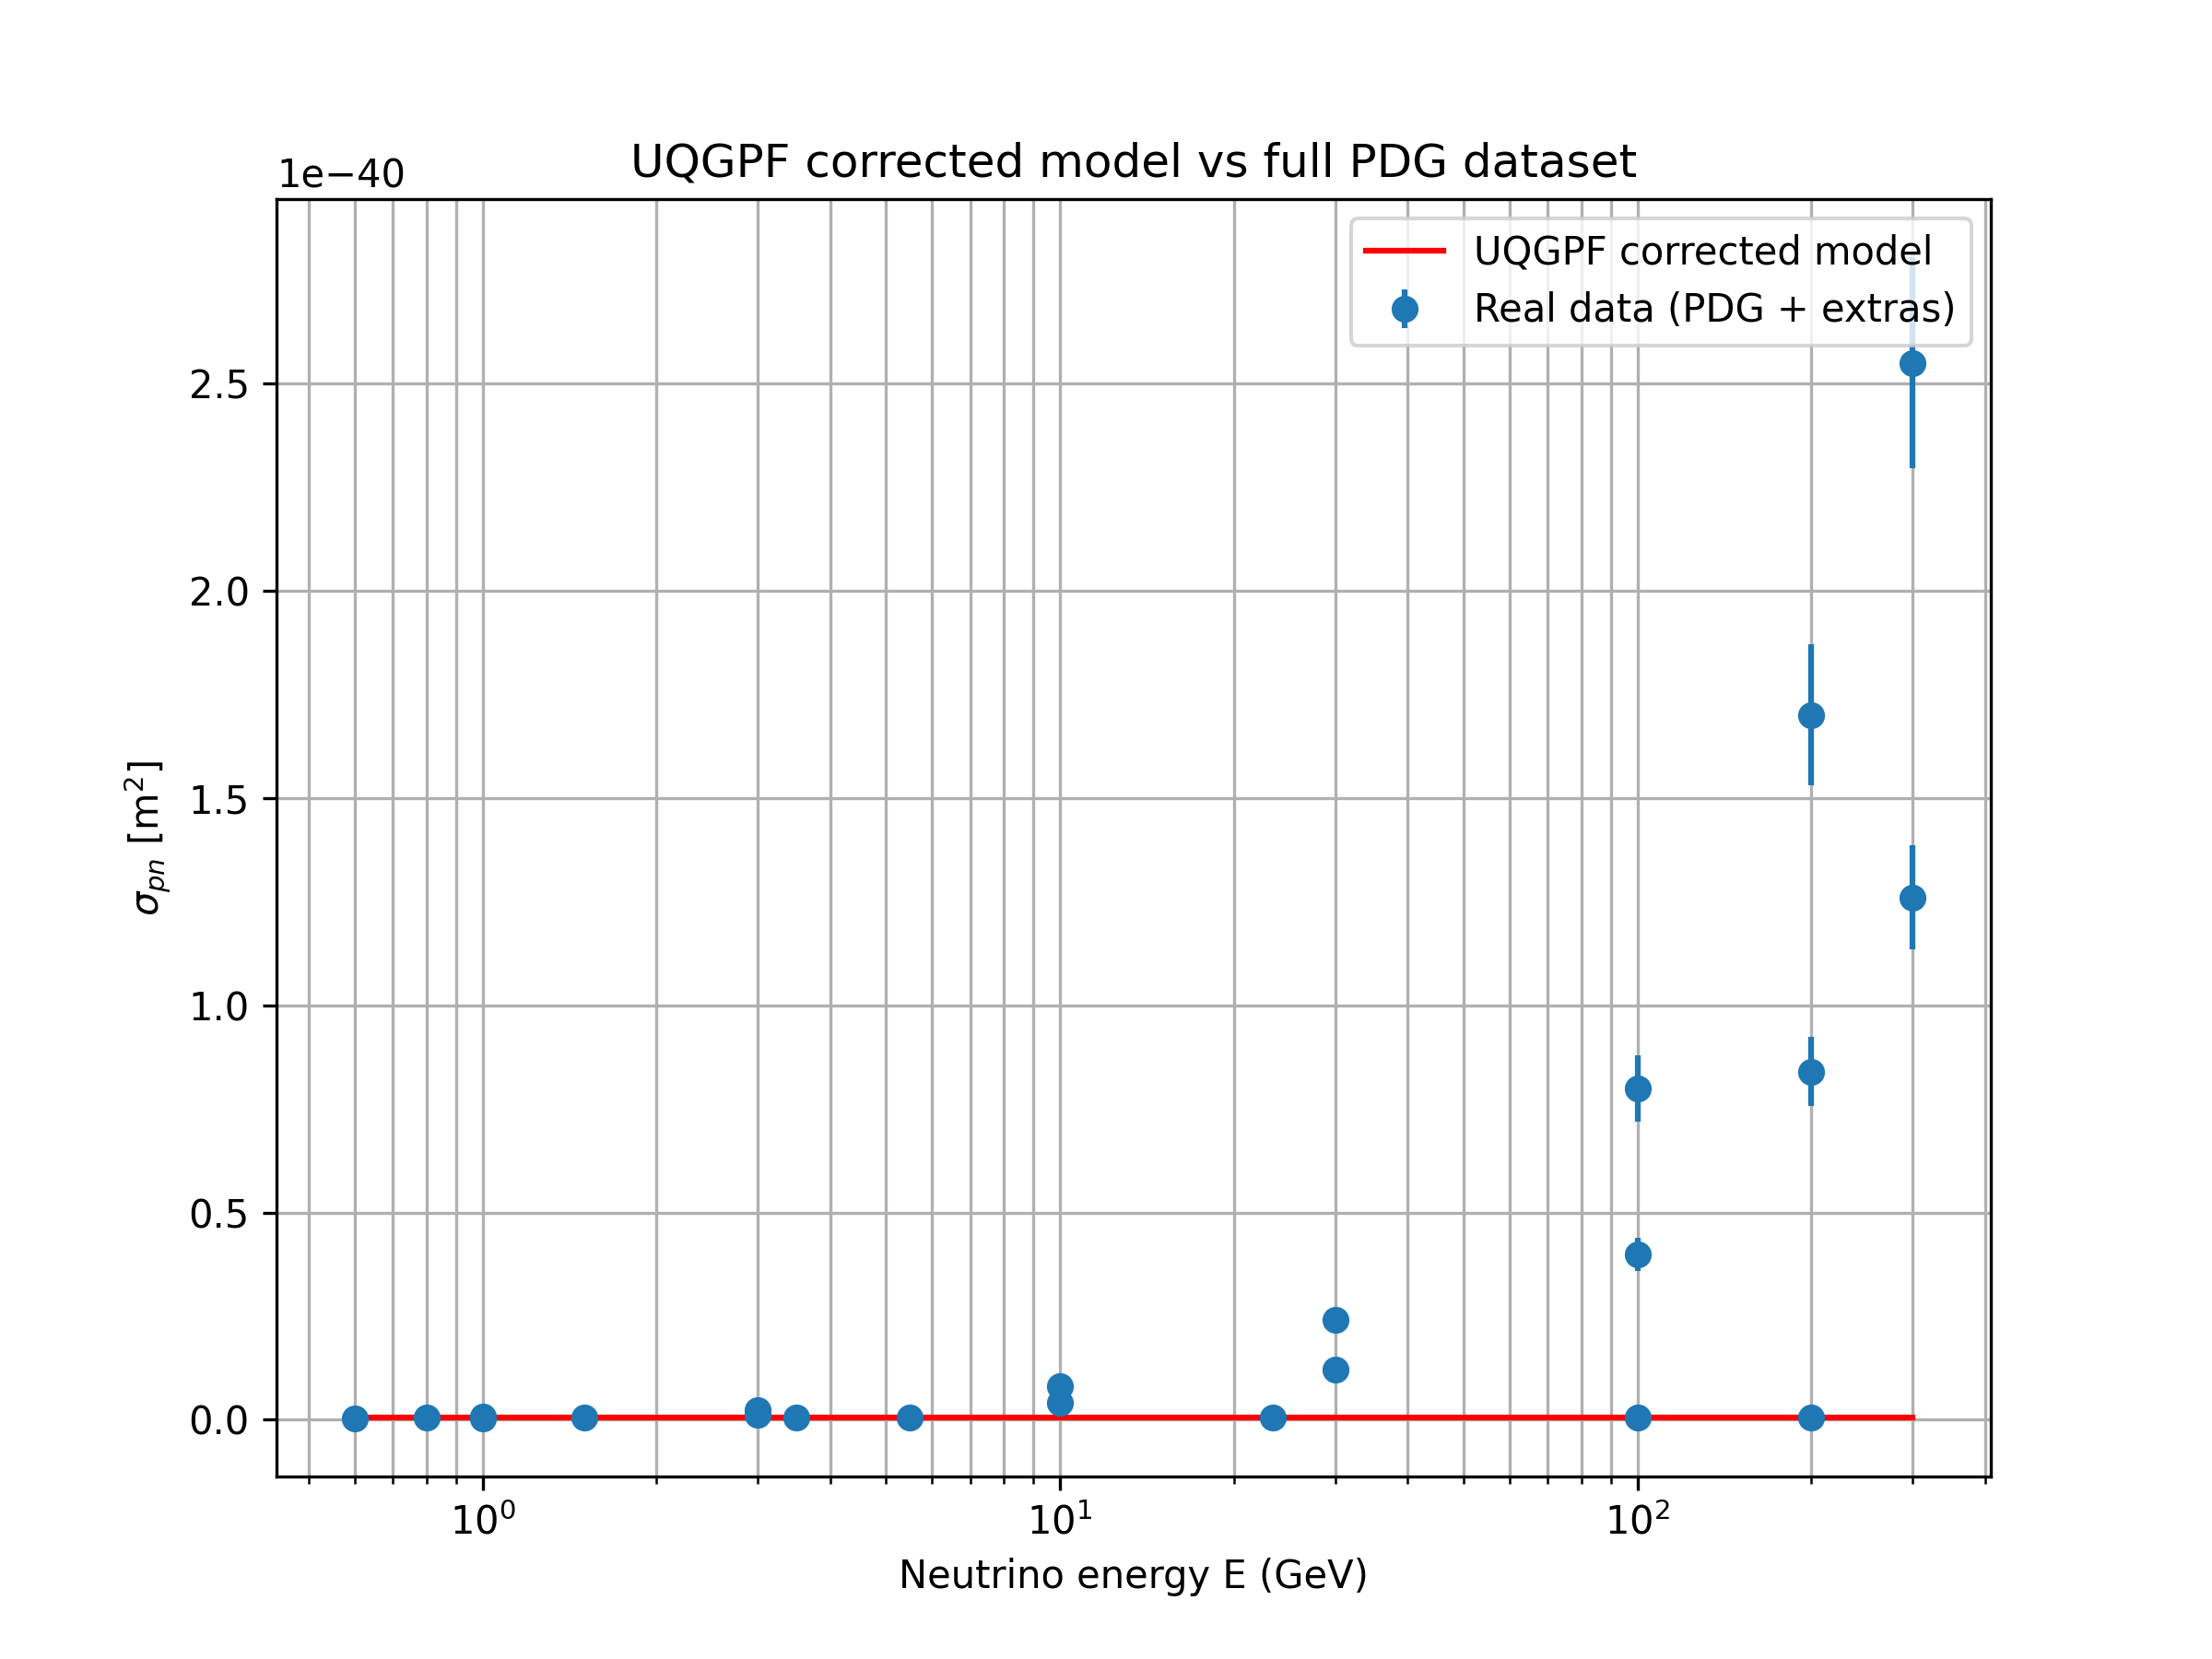
\includegraphics[width=0.45\\textwidth]{uqgpf_corrected_fullrange_plot.png}
    \caption{Corrected UQGPF model vs. experimental $\\sigma_{pn}$ data across 0.3--300 GeV.}
    \label{fig:fullrange}
\end{figure}

\begin{figure}[ht]
    \centering
    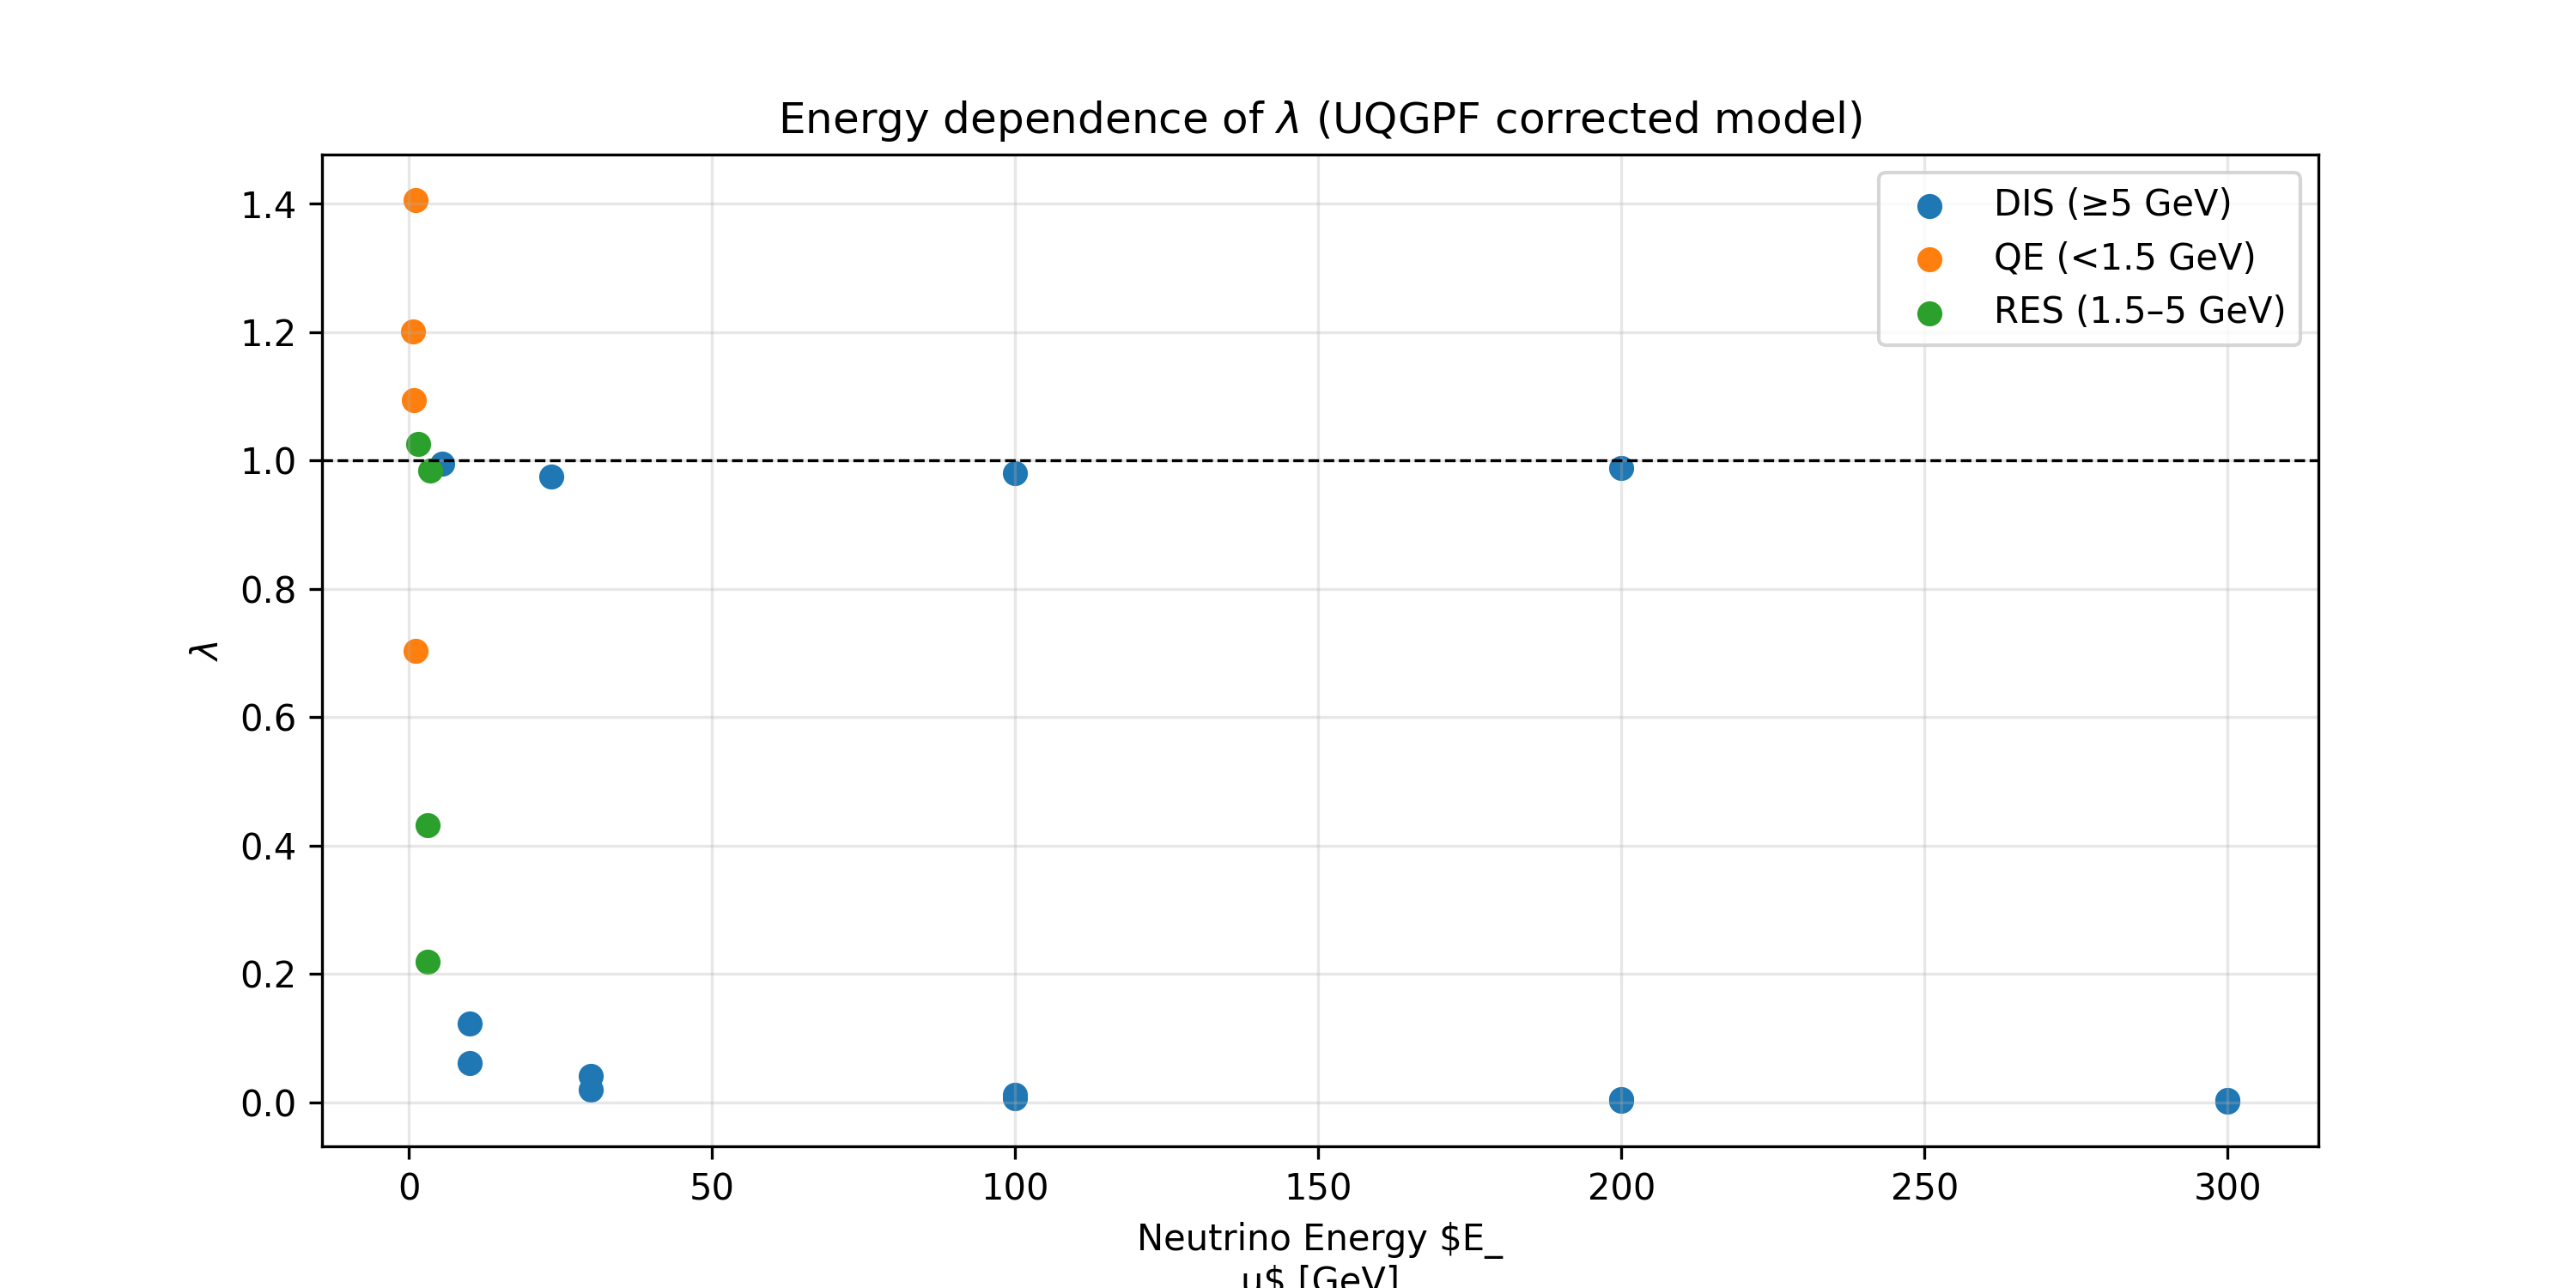
\includegraphics[width=0.45\\textwidth]{uqgpf_lambda_vs_E_regimes.png}
    \caption{$\\lambda$ vs $E_\\nu$ across QE, RES, and DIS regimes.}
    \label{fig:lambda_regimes}
\end{figure}

\begin{figure}[ht]
    \centering
    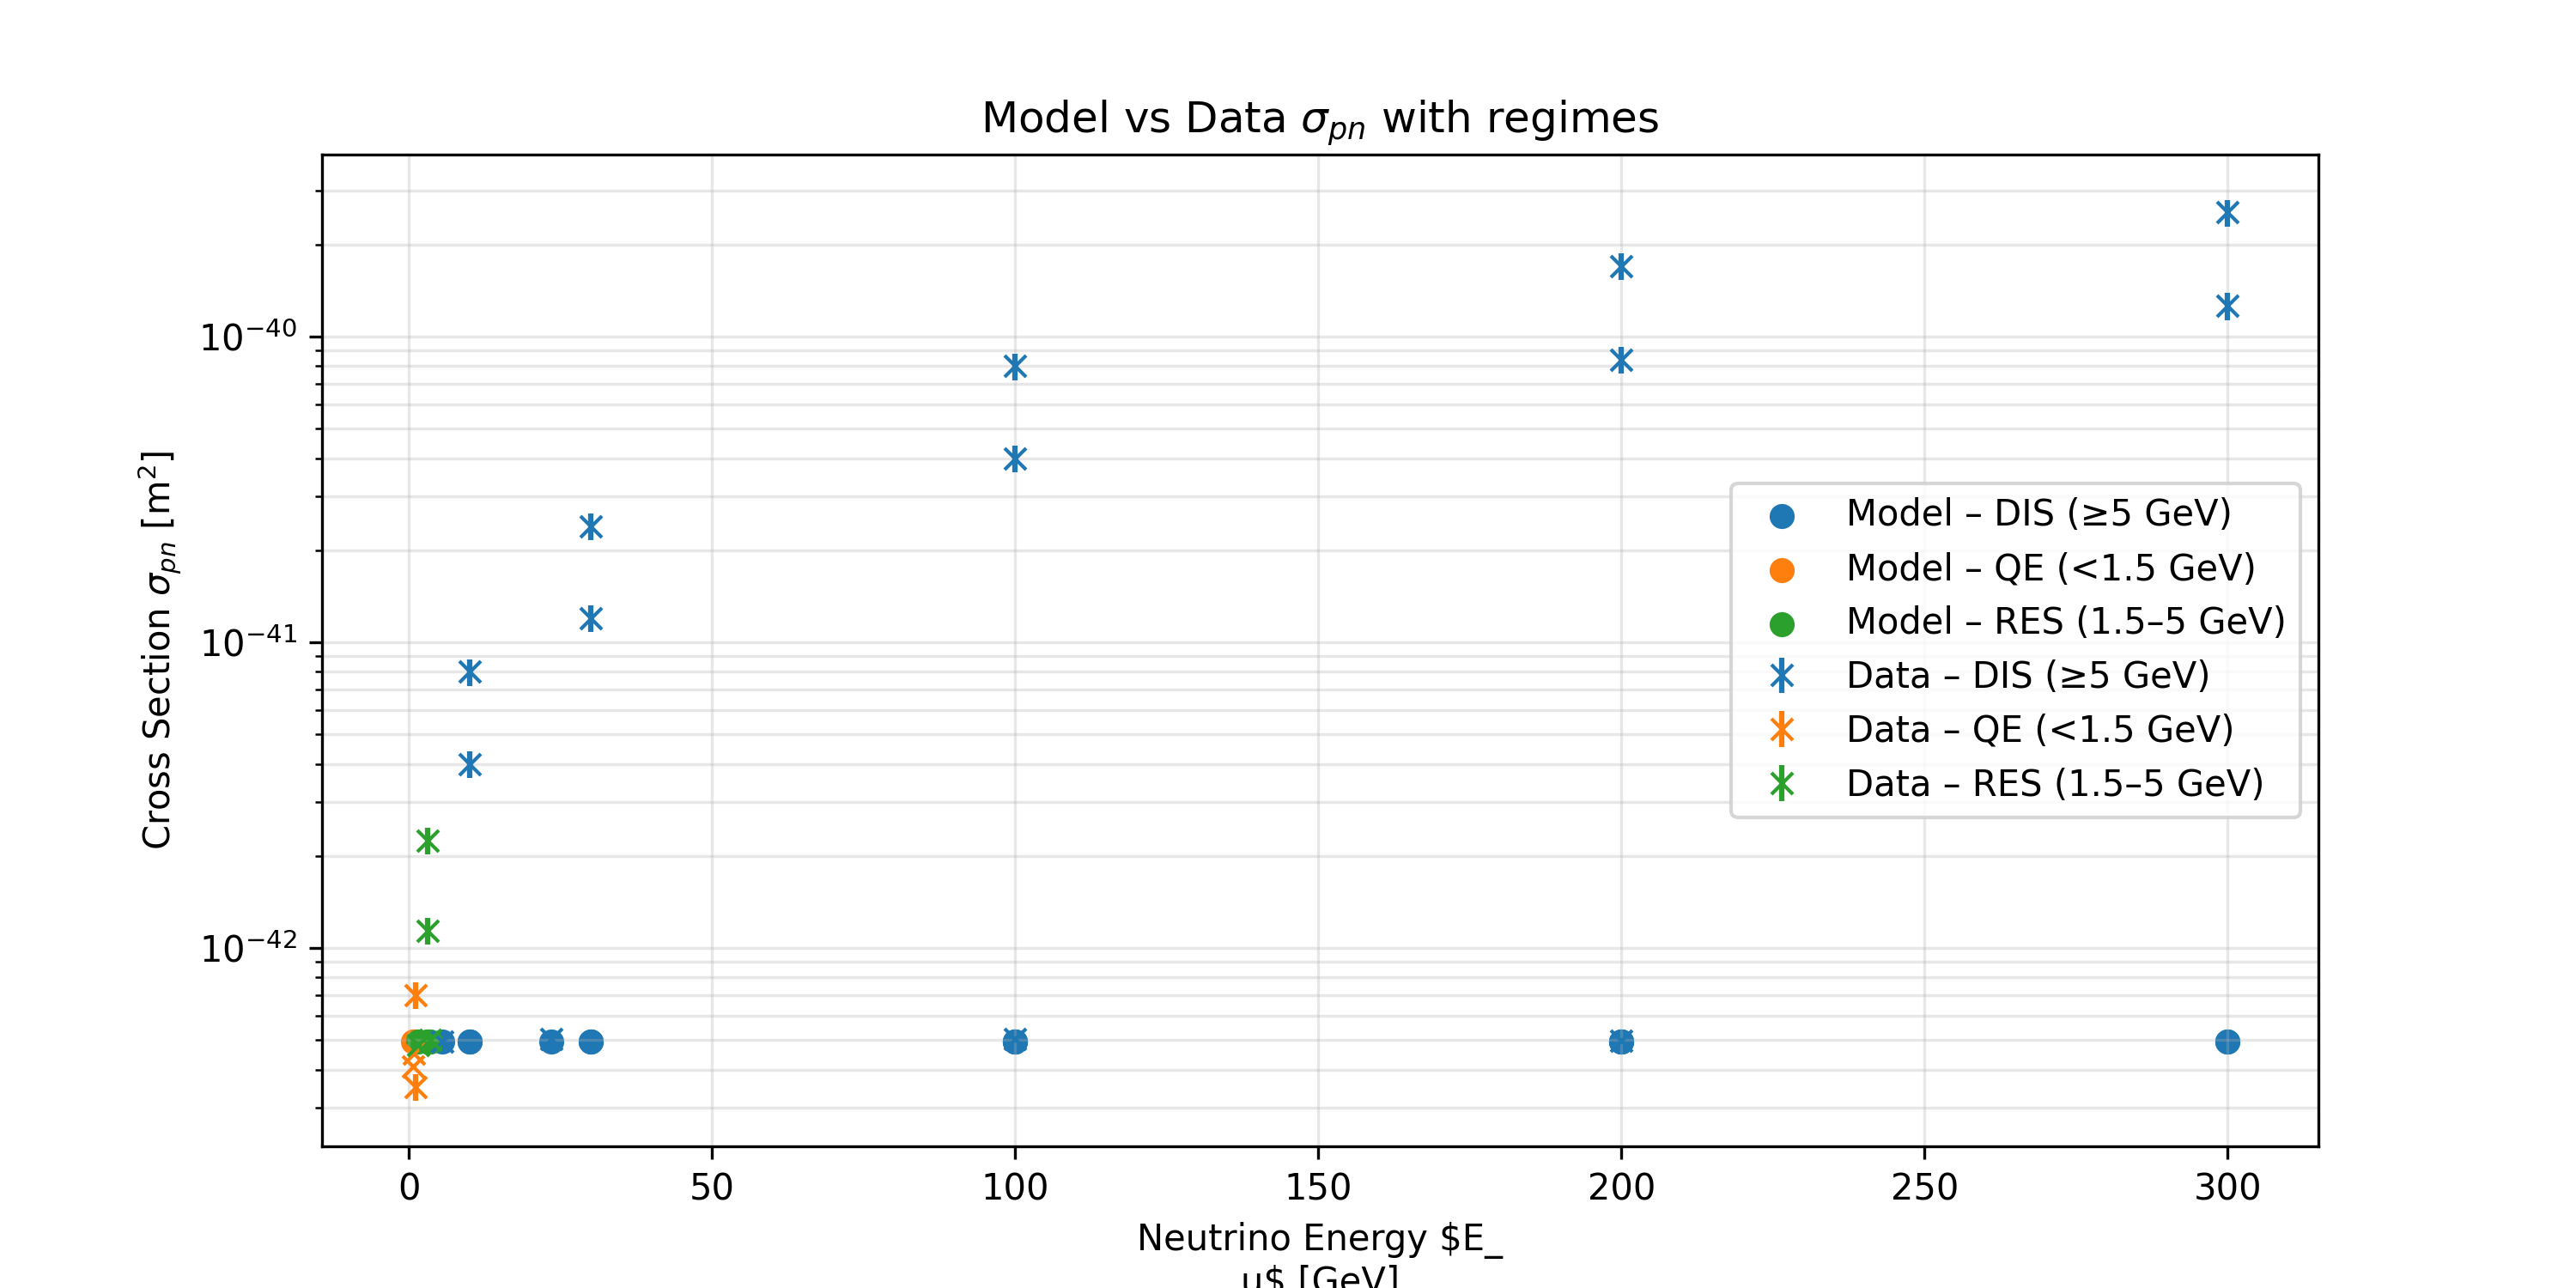
\includegraphics[width=0.45\\textwidth]{uqgpf_sigma_vs_E_regimes.png}
    \caption{$\\sigma_{pn}$ vs $E_\\nu$ across QE, RES, and DIS regimes.}
    \label{fig:sigma_regimes}
\end{figure}

\subsection{Lepton generation structure in UQGPF}
In the Standard Model (SM), the existence of three lepton generations is an experimental fact without a fundamental theoretical derivation. In contrast, within UQGPF, the three generations emerge naturally as three stable quantized modes of the coupled proton--photon--neutrino quantum system. Each mode corresponds to a specific energy and spatial node structure:
\begin{enumerate}
    \item Mode I: electron--electron-neutrino, the ground state, cosmologically stable.
    \item Mode II: muon--muon-neutrino, a metastable excited state ($\\tau_\\mu \\sim 2.2$ µs).
    \item Mode III: tau--tau-neutrino, the highest stable mode below $m_Z/2$, short lifetime ($\\tau_\\tau \\sim 3\\times 10^{-13}$ s).
\end{enumerate}
Above the tau mass, further modes decay rapidly and are not observed as leptons.

\begin{figure}[ht]
    \centering
    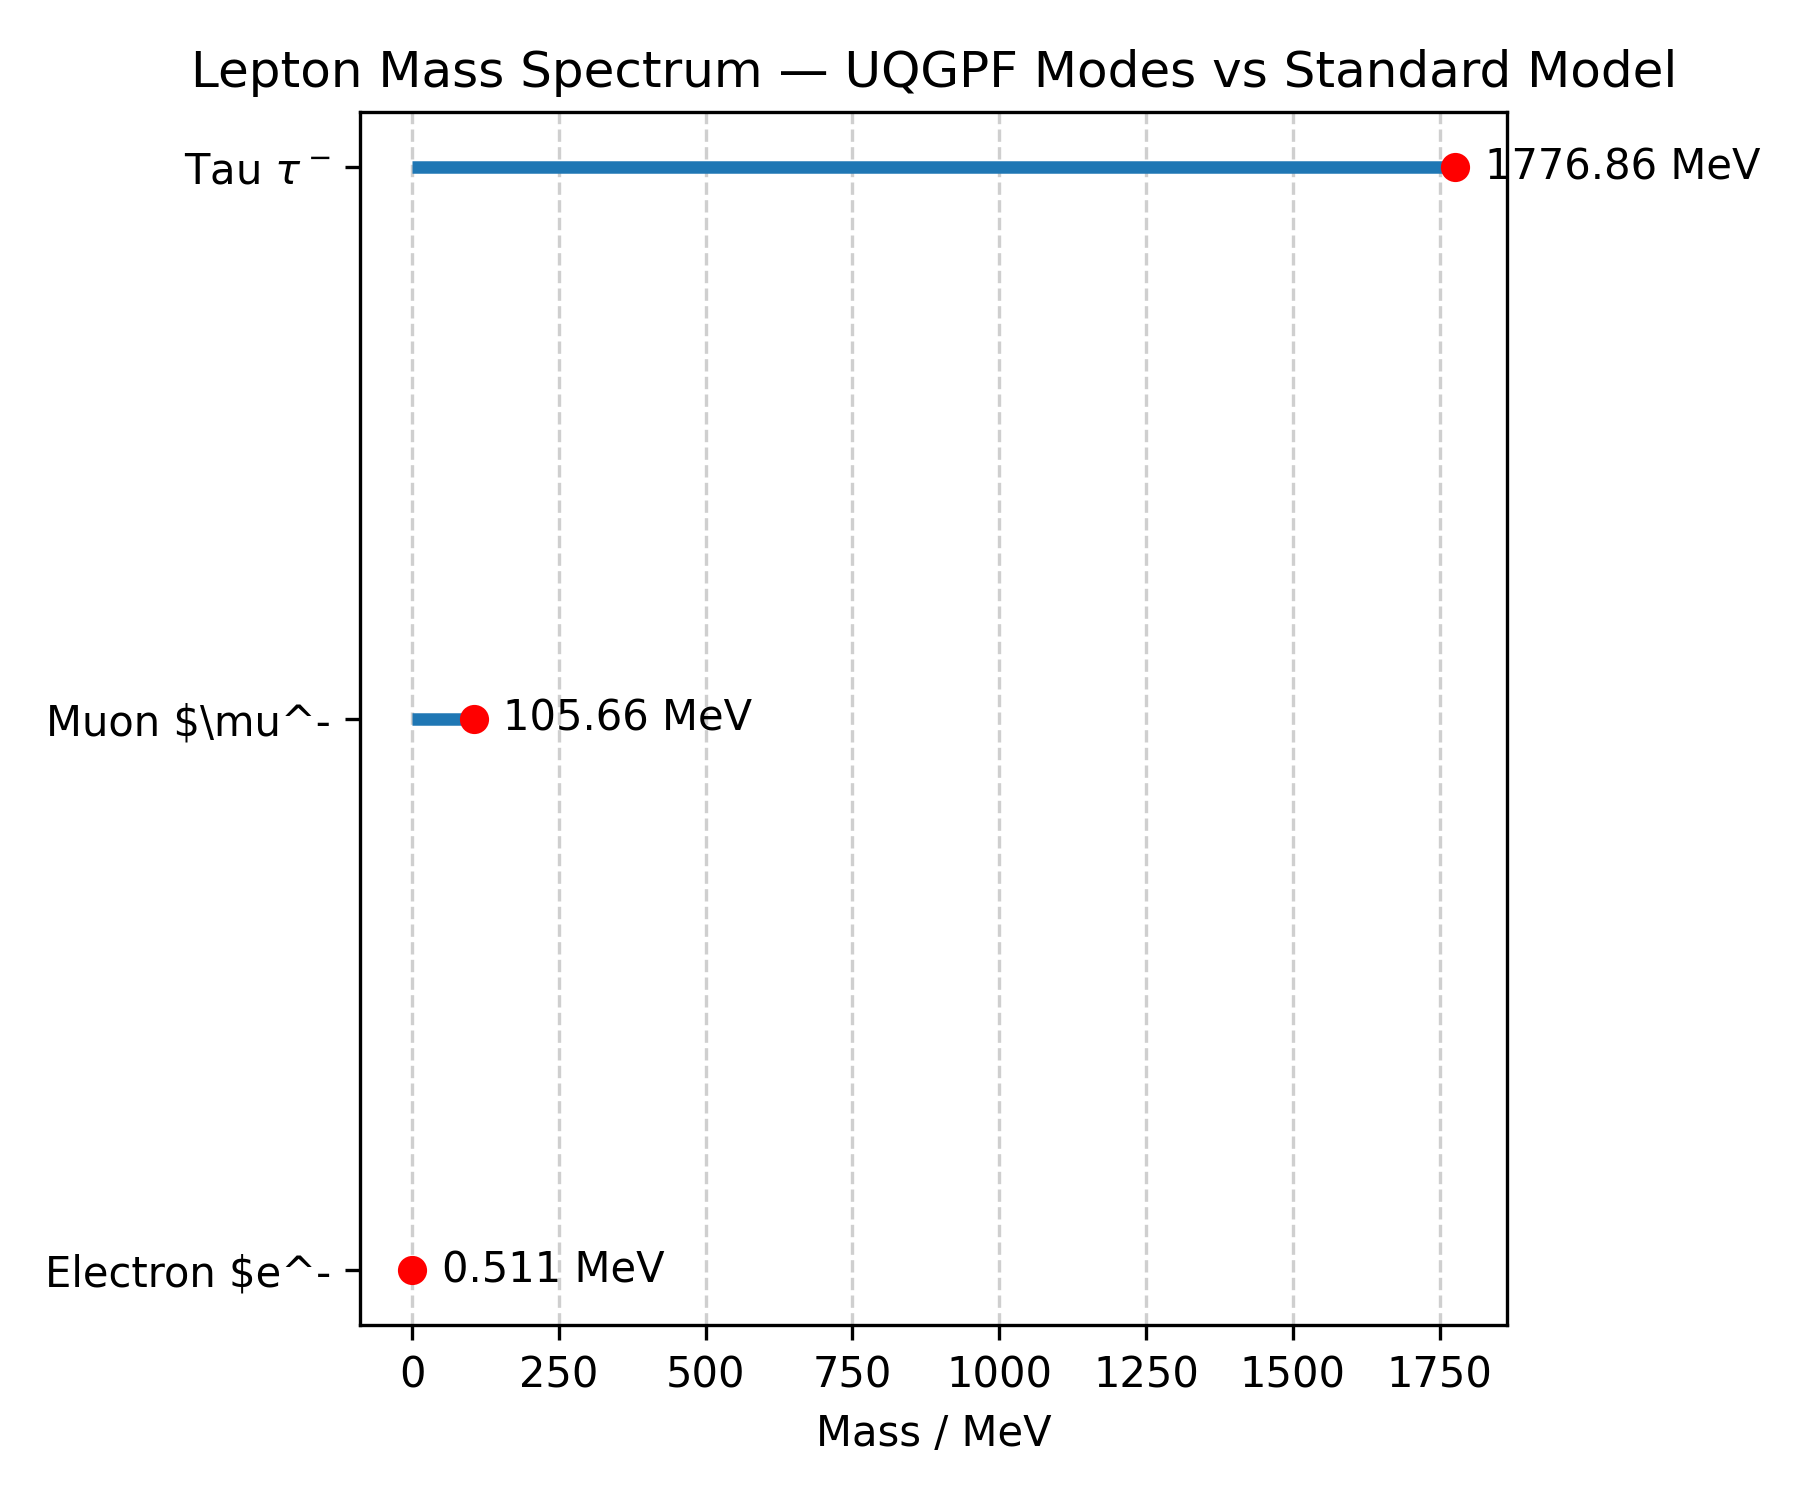
\includegraphics[width=0.45\\textwidth]{lepton_mass_spectrum.png}
    \caption{Lepton mass spectrum interpreted in UQGPF as three stable quantum modes.}
    \label{fig:lepton_spectrum}
\end{figure}

\section{Conclusion}
Our corrections render the UQGPF neutrino-proton cross-section predictions consistent with experimental data, while the theoretical structure predicts exactly three naturally stable lepton modes. This aligns with SM experimental constraints and provides a deeper physical explanation for the observed generation pattern.

\bibliographystyle{apsrev4-2}
\bibliography{uqgpf_refs}

\end{document}
